\chapter{Metodolog\'ia}
\label{cap:metodologia}

Este cap\'itulo describe el dise\~no experimental empleado para responder a los objetivos
del \cref{cap:introduccion}. En primer lugar, expone el planteamiento comparativo y las
variables implicadas. A continuaci\'on, detalla la tarea, el conjunto de datos y la
arquitectura de la pol\'itica. Por \'ultimo, define las cinco variantes evaluadas, los
protocolos de entrenamiento y evaluaci\'on, las m\'etricas, el entorno de ejecuci\'on y el
coste temporal de los experimentos.

\section{Planteamiento experimental}
\label{sec:planteamiento}

El estudio adopta un dise\~no comparativo centrado en una variable de inter\'es. Esa variable
es el bloque visual de la pol\'itica, entendido como el codificador, sus pesos y su cadena de
preprocesado. La arquitectura generativa, los datos y la evaluaci\'on permanecen constantes;
el presupuesto y el tama\~no de lote presentan las desviaciones descritas en el
\cref{sec:protocolo}.

El planteamiento parte de tres \textbf{expectativas previas}, no de hip\'otesis
estad\'isticas. La distinci\'on es deliberada: una hip\'otesis sobre estrategias de
entrenamiento exigir\'ia varias ejecuciones por estrategia, y este dise\~no dispone de una
sola. Las expectativas se enuncian, por tanto, sobre las configuraciones completas que se
comparan, y su papel es orientar la lectura de los resultados, no ser sometidas a
contraste formal.

\begin{enumerate}[label=E\arabic*.,leftmargin=*]
  \item Las configuraciones cuyo codificador parte de pesos preentrenados sobre un corpus
        amplio de im\'agenes superar\'an a la configuraci\'on entrenada desde cero, puesto
        que el n\'umero de demostraciones disponibles es reducido.
  \item Entre las dos configuraciones que comparten arquitectura ResNet-18 preentrenada,
        la que actualiza los pesos del codificador superar\'a a la que los mantiene
        congelados, al adaptar la representaci\'on a la distribuci\'on visual sint\'etica
        de la tarea.
  \item Las configuraciones basadas en transformador de visi\'on (\textit{Vision
        Transformer}, ViT) presentar\'an un coste de inferencia del codificador superior
        al de las convolucionales. El orden interno entre las cuatro configuraciones
        preentrenadas se deja abierto: el dise\~no no incluye margen de equivalencia ni
        prueba dirigida a demostrarlo, de modo que ese orden puede quedar sin resolver.
\end{enumerate}

El \cref{sec:contraste-hipotesis} recupera las tres expectativas y las confronta con la
evidencia obtenida, indicando en cada caso el nivel al que la afirmaci\'on resulta
sostenible.

Para que la comparaci\'on resulte interpretable, se mantienen constantes cinco factores: la
red generativa y sus hiperpar\'ametros, el conjunto de datos y su partici\'on, la semilla de
entrenamiento, el protocolo de evaluaci\'on y la dimensi\'on del vector de condicionamiento
a la salida del codificador.
Esta \'ultima restricci\'on resulta esencial: todas las variantes entregan un vector de
\num{512} componentes, de modo que la red generativa recibe siempre una entrada de la misma
dimensi\'on.

A esos factores constantes se suma una \textbf{premisa de dise\~no} que conviene enunciar
antes que ning\'un resultado: cada variante se entrena una sola vez, con la semilla
\num{42}. La premisa responde al reparto del presupuesto de c\'omputo. Una ejecuci\'on
ocupa entre \num{11} y \num{96} horas de la \'unica unidad de procesamiento gr\'afico
(\textit{Graphics Processing Unit}, GPU) disponible y las cinco suman \SI{237.1}{\hour},
seg\'un el \cref{sec:coste}; con tres semillas por variante el c\'omputo rondar\'ia las
\SI{700}{\hour}, incompatibles con el calendario del trabajo. Ante la alternativa entre
cubrir cinco bloques visuales con una semilla o dos bloques con tres semillas, se opt\'o
por la cobertura.

La consecuencia es directa y determina toda la especificaci\'on estad\'istica del
\cref{sec:seleccion-prueba}: la unidad experimental sobre la que se infiere es el
artefacto entrenado, es decir, el punto de control resultante, y no la estrategia de
entrenamiento que lo produjo. Los contrastes de este trabajo comparan cinco puntos de
control fijos ante nuevas condiciones iniciales; no cuantifican la variabilidad que
introducir\'ia volver a entrenar la misma configuraci\'on con otra semilla. Toda lectura
de los resultados debe respetar ese nivel.

\section{Tarea y conjunto de datos}
\label{sec:datos}

La tarea de evaluaci\'on es Push-T, propuesta junto con \textit{Diffusion Policy}
\cite{chi2025diffusion}. Un efector circular debe empujar una pieza r\'igida con forma de T
sobre un plano hasta hacerla coincidir con una silueta objetivo. La tarea exige contacto
intermitente y admite varias secuencias de empuje v\'alidas, de ah\'i su car\'acter
multimodal.

La pol\'itica observa dos modalidades: una imagen en color de \num{96}$\times$\num{96}
p\'ixeles renderizada desde una vista cenital y la posici\'on bidimensional del efector. La
acci\'on es la posici\'on objetivo del efector, es decir, se emplea control en posici\'on y
no en velocidad. El entorno resuelve la din\'amica de contacto mediante un motor de
cuerpos r\'igidos bidimensional.

El conjunto de datos es el publicado por los autores del m\'etodo, en formato \texttt{zarr}
y con un tama\~no aproximado de \num{30} megabytes. Contiene \num{206} demostraciones
teleoperadas por un operador humano, que suman \num{25650} transiciones. Cada transici\'on
almacena la imagen, el estado del efector, los puntos caracter\'isticos de la pieza, la
acci\'on ejecutada y el n\'umero de contactos.

Cada demostraci\'on arranca en la condici\'on inicial que el simulador genera a partir de
una semilla propia, y esas semillas recorren los valores de \num{0} a \num{205}. El dato se
ha verificado reproduciendo con el entorno el primer instante de las \num{206}
demostraciones, que se recupera sin error apreciable. Las semillas reservadas para la
evaluaci\'on, descritas en el \cref{sec:evaluacion}, quedan por tanto fuera de ese rango.

La partici\'on de los datos reproduce la de la implementaci\'on de referencia y se resume en
la \cref{tab:particion}. Un sorteo aleatorio reserva el dos por ciento de los episodios para
validaci\'on, cuatro en total, y un segundo sorteo escoge \num{90} de los \num{202}
restantes para el entrenamiento. Los \num{112} episodios no seleccionados, el
\SI{54.4}{\percent} del conjunto, no intervienen en el ajuste. La semilla de ambos sorteos
est\'a fijada en \num{42} dentro de la configuraci\'on de la tarea y es independiente de la
semilla de entrenamiento, de modo que las cinco variantes emplean exactamente los mismos
episodios.

\begin{table}[htbp]
  \centering
  \caption{Reparto del conjunto de demostraciones de Push-T y caracter\'isticas de cada
    subconjunto. La puntuaci\'on es la que alcanza el operador humano seg\'un la
    \cref{eq:score}.}
  \label{tab:particion}
  \small
  \begin{tabular}{lrrrrr}
    \toprule
    Subconjunto & Episodios & Transiciones & Ventanas & Longitud media &
      Puntuaci\'on media \\
    \midrule
    Entrenamiento & 90  & \num{11356} & \num{10726} & \num{126.2} & \num{0.894} \\
    Validaci\'on  & 4   & \num{432}   & \num{404}   & \num{108.0} & \num{0.893} \\
    Descartados   & 112 & \num{13862} & ---         & \num{123.8} & \num{0.891} \\
    \midrule
    Total         & 206 & \num{25650} & ---         & \num{124.5} & \num{0.892} \\
    \bottomrule
  \end{tabular}
  \fuente{elaboraci\'on propia}
\end{table}

El tope de \num{90} episodios procede de la implementaci\'on de referencia y define el
r\'egimen de pocas demostraciones que motiva las expectativas del
\cref{sec:planteamiento}.
Ese r\'egimen admite una descripci\'on cuantitativa. Los episodios de entrenamiento aportan
\num{11356} transiciones, equivalentes a \SI{18.9}{\minute} de teleoperaci\'on de los
\SI{42.8}{\minute} que contiene el fichero. Con el horizonte de \num{16} instantes, el
muestreador extrae de ellos \num{10726} ventanas, que a lote efectivo \num{64} producen
\num{168} actualizaciones por \'epoca.

La calidad de las demostraciones acota lo que la pol\'itica puede aprender. Al aplicar a
cada una la m\'etrica definida en el \cref{sec:metricas}, el operador humano obtiene una
puntuaci\'on media de \num{0.892}, con mediana \num{0.896} y recorrido entre \num{0.813} y
\num{0.949}. Ninguna de las \num{206} demostraciones alcanza el umbral de cobertura que el
entorno considera un \'exito, de manera que el valor unitario de la m\'etrica no est\'a
representado en los datos. Esa cifra es una referencia y no una cota superior estricta,
puesto que las condiciones iniciales de las demostraciones no coinciden con las de la
evaluaci\'on.

La \cref{fig:caracterizacion-dataset} re\'une las cuatro distribuciones que describen el
conjunto: longitud de los episodios, puntuaci\'on del demostrador, posici\'on inicial de la
pieza y orientaci\'on inicial de la pieza.

\begin{figure}[htbp]
  \centering
  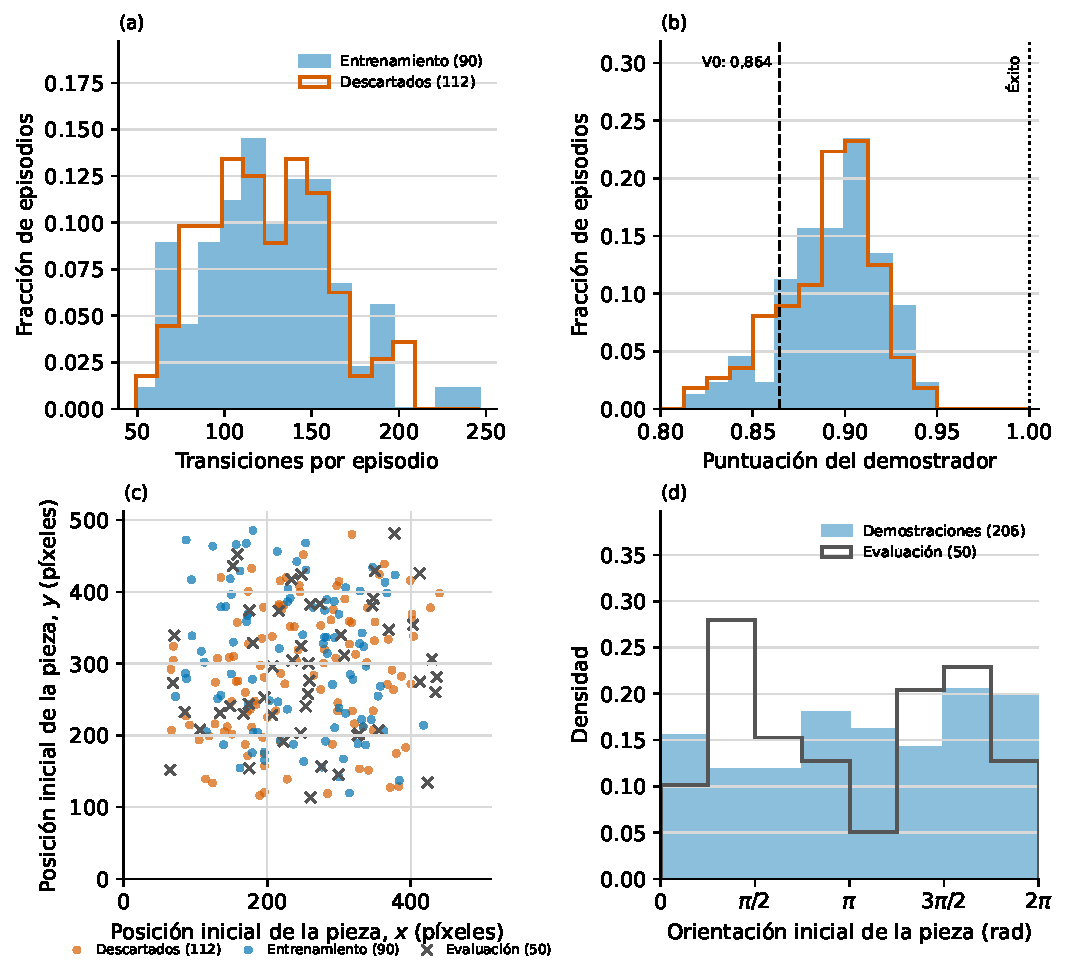
\includegraphics[width=\textwidth]{img/caracterizacion_dataset.pdf}
  \caption[Caracterizaci\'on del conjunto de demostraciones de
    Push-T.]{Caracterizaci\'on del conjunto de demostraciones de Push-T: (a) longitud de los
    episodios; (b) puntuaci\'on del demostrador, con el m\'aximo de V0 y el umbral de
    \'exito; (c) posici\'on inicial de la pieza, con las \num{50} condiciones de
    evaluaci\'on superpuestas; (d) orientaci\'on inicial de la pieza.}
  \label{fig:caracterizacion-dataset}
  \fuente{elaboraci\'on propia}
\end{figure}

El argumento que descarta un sesgo de selecci\'on es el procedimiento, no una prueba
estad\'istica: el reparto responde a un sorteo aleatorio uniforme sobre los \'indices de
episodio, sin ning\'un criterio de calidad, longitud ni dificultad. Un sorteo uniforme no
puede introducir sesgo sistem\'atico por construcci\'on.

Las comparaciones entre los dos subconjuntos cumplen aqu\'i un papel distinto y m\'as
modesto, el de comprobaci\'on descriptiva de que el sorteo se ejecut\'o como se describe.
Se presentan como tama\~nos de efecto con su incertidumbre, y no como valores $p$, porque
no rechazar la igualdad no demuestra equivalencia. Los episodios de entrenamiento son, en
media, \num{2.4} transiciones m\'as largos que los descartados, con un intervalo BCa al
\SI{95}{\percent} de {[\num{-7.7};\,\num{12.6}]} sobre una longitud media de \num{126}, es
decir menos del \SI{10}{\percent} de esa media en cualquiera de los dos extremos. En
puntuaci\'on del demostrador la diferencia es de \num{0.004}, con intervalo
{[\num{-0.004};\,\num{0.011}]}, un orden de magnitud por debajo de las diferencias entre
variantes que este trabajo interpreta. El $\delta$ de Cliff, que mide la probabilidad de
que un episodio de un subconjunto supere a uno del otro, vale \num{0.026} en longitud y
\num{0.085} en puntuaci\'on, ambos dentro de lo que se considera un efecto despreciable.
El mismo criterio se aplica a la comparaci\'on entre las condiciones iniciales de
entrenamiento y las \num{50} de evaluaci\'on, superpuestas en la
\cref{fig:caracterizacion-dataset}: los estad\'isticos de Kolmogorov-Smirnov sobre la
posici\'on del efector, la posici\'on de la pieza y su orientaci\'on quedan entre
\num{0.232} y \num{0.696} en valor $p$, sin que de ello se concluya equivalencia. En
cambio, el efecto de aprovechar tambi\'en los \num{112} episodios descartados no se ha
medido y queda recogido en el \cref{sec:trabajo-futuro}.

La procedencia p\'ublica del conjunto no sustituye a la comprobaci\'on del archivo
concreto que se ha utilizado. La \cref{tab:integridad} recoge los controles de integridad
aplicados sobre \'el, junto con la huella que lo identifica de forma un\'ivoca.

\begin{table}[htbp]
  \centering
  \caption{Controles de integridad del archivo de demostraciones.}
  \label{tab:integridad}
  \small
  \begin{tabular}{lll}
    \toprule
    Control & Regla & Resultado \\
    \midrule
    Valores ausentes  & Ning\'un \texttt{NaN} en los cinco arreglos & \num{0} \\
    Valores infinitos & Ning\'un \texttt{Inf} en los cinco arreglos & \num{0} \\
    Longitud coherente & Todos los arreglos con \num{25650} filas & Cumple \\
    \'Indices de episodio & Estrictamente crecientes, \num{206} finales & Cumple \\
    Longitud de episodio & Entre \num{49} y \num{246} transiciones & Cumple \\
    Rango de la acci\'on & Coordenadas en $[\num{12};\ \num{511}]$ p\'ixeles & Cumple \\
    Rango del estado & Coordenadas en $[\num{0.0002};\ \num{510.96}]$ & Cumple \\
    Rango de la imagen & Intensidades en $[\num{65};\ \num{255}]$, \texttt{float32}
      & Cumple \\
    Estados duplicados & Filas de \texttt{state} repetidas & \num{0} \\
    Tama\~no en disco & Suma de los bloques del directorio & \SI{31.0}{\mega\byte} \\
    \bottomrule
  \end{tabular}
  \notatabla{Los controles se ejecutan sobre el propio archivo \texttt{zarr}, abierto en
    modo lectura y recorrido por bloques para no cargar en memoria los \SI{2.84}{\giga\byte}
    del arreglo de im\'agenes. La huella SHA-256 del \'arbol de ficheros, calculada sobre
    su contenido en orden determinista, es
    \texttt{c235ab79\dots 275e36a4}; el valor completo figura en la
    \cref{tab:identificadores}.}
  \fuente{elaboraci\'on propia}
\end{table}

Conviene precisar, por \'ultimo, que la evaluaci\'on no consume datos de este fichero. El
rendimiento se mide ejecutando la pol\'itica en el simulador sobre condiciones iniciales
generadas de forma independiente, seg\'un se detalla en el \cref{sec:evaluacion}.

\section{Arquitectura de la pol\'itica}
\label{sec:arquitectura}

\textit{Diffusion Policy} modela la distribuci\'on condicional
$p(\mathbf{A}_t \mid \mathbf{O}_t)$, donde $\mathbf{O}_t$ agrupa las observaciones de los
\'ultimos $T_o$ instantes y $\mathbf{A}_t$ es una secuencia de $T_p$ acciones futuras
\cite{chi2025diffusion}. El muestreo de esa distribuci\'on se realiza mediante un modelo
probabil\'istico de difusi\'on con eliminaci\'on de ruido (\textit{Denoising Diffusion
Probabilistic Model}, DDPM) \cite{ho2020ddpm}.

El planificador de ruido fija una sucesi\'on $\beta_1,\dots,\beta_K$ y, a partir de ella,
$\alpha_k = 1-\beta_k$ y $\bar{\alpha}_k = \prod_{j=1}^{k}\alpha_j$. El proceso directo
perturba una secuencia de acciones real $\mathbf{A}^0_t$ interpolando entre la se\~nal
limpia y ruido gaussiano $\epsilon\sim\mathcal{N}(0,\mathbf{I})$, con los coeficientes que
recoge la \cref{eq:proceso-directo} del \cref{cap:estado-del-arte}:

\begin{equation}
  \mathbf{A}^{k}_t = \sqrt{\bar{\alpha}_k}\,\mathbf{A}^0_t
    + \sqrt{1-\bar{\alpha}_k}\;\epsilon .
  \label{eq:perturbacion}
\end{equation}

La red $\epsilon_\theta$ se ajusta para predecir ese ruido a partir del estado perturbado,
del \'indice de paso y de la observaci\'on. La funci\'on de p\'erdida es el error
cuadr\'atico medio sobre el ruido, recogido en la \cref{eq:perdida}.

\begin{equation}
  \mathcal{L} = \mathbb{E}_{k,\,\epsilon}\left[\left\lVert \epsilon -
    \epsilon_\theta\!\left(\mathbf{O}_t,\;
      \sqrt{\bar{\alpha}_k}\,\mathbf{A}^0_t + \sqrt{1-\bar{\alpha}_k}\,\epsilon,\; k\right)
    \right\rVert^2\right]
  \label{eq:perdida}
\end{equation}

En la \cref{eq:perdida}, el \'indice $k$ se muestrea de forma uniforme en
$\{1,\dots,K\}$ y determina, a trav\'es de $\bar{\alpha}_k$, la magnitud del ruido
inyectado. La observaci\'on $\mathbf{O}_t$ act\'ua como condicionamiento, no como variable
generada, lo que reduce el coste de inferencia. Por tanto, la calidad de la
representaci\'on visual condiciona directamente lo que la red generativa puede aprender.

Durante la inferencia, la pol\'itica parte de una secuencia de ruido puro
$\mathbf{A}^K_t\sim\mathcal{N}(0,\mathbf{I})$ y aplica $K$ transiciones inversas seg\'un la
\cref{eq:muestreo}.

\begin{equation}
  \mathbf{A}^{k-1}_t = \frac{1}{\sqrt{\alpha_k}}\left(\mathbf{A}^{k}_t -
    \frac{\beta_k}{\sqrt{1-\bar{\alpha}_k}}\;
    \epsilon_\theta\!\left(\mathbf{O}_t,\, \mathbf{A}^{k}_t,\, k\right)\right)
    + \sigma_k\,\mathbf{z},
  \qquad \mathbf{z}\sim\mathcal{N}(0,\mathbf{I})
  \label{eq:muestreo}
\end{equation}

La \cref{eq:muestreo} es la forma concreta que adoptan los coeficientes gen\'ericos
$\alpha$, $\gamma$ y $\sigma$ del muestreo DDPM: $\alpha = \alpha_k^{-1/2}$,
$\gamma = \beta_k(1-\bar{\alpha}_k)^{-1/2}$ y, con la varianza fija menor que emplea la
configuraci\'on de este trabajo,
$\sigma_k^2 = \tfrac{1-\bar{\alpha}_{k-1}}{1-\bar{\alpha}_k}\,\beta_k$. El t\'ermino
$\mathbf{z}$ se anula en el \'ultimo paso, $k=1$. El ruido fresco que se a\~nade en los
dem\'as preserva el car\'acter estoc\'astico del muestreo y, con ello, la capacidad de
representar varios modos de acci\'on.

El planificador concreto es el DDPM con $K = \num{100}$ pasos, id\'entico en entrenamiento
y en inferencia, sin acelerarlo mediante muestreadores impl\'icitos. Su sucesi\'on de
$\beta_k$ sigue el plan de coseno al cuadrado, definido por
$\bar{\alpha}_k = f(k)/f(0)$ con
$f(k) = \cos^2\!\left(\tfrac{k/K + s}{1+s}\cdot\tfrac{\pi}{2}\right)$ y
$s = 0{,}008$, y los $\beta_k$ resultantes se acotan superiormente en $0{,}999$ para
evitar la singularidad final. La red predice el ruido y no la muestra limpia, y la
estimaci\'on intermedia de $\mathbf{A}^0_t$ se recorta al intervalo $[-1,1]$ en el que se
normalizan las acciones. Con este plan, los par\'ametros de inicio y fin de una
progresi\'on lineal de $\beta$ no intervienen.

Las acciones generadas se aplican bajo un esquema de horizonte deslizante. La pol\'itica
recibe $T_o = 2$ observaciones, predice $T_p = 16$ acciones y ejecuta \'unicamente las
$T_a = 8$ primeras antes de replanificar \cite{chi2025diffusion}. Esta configuraci\'on
equilibra la consistencia temporal de la trayectoria con la capacidad de reaccionar ante
cambios en la escena.

La red $\epsilon_\theta$ es una red convolucional unidimensional con arquitectura en U y
dimensiones de canal \num{512}, \num{1024} y \num{2048} en sus tres niveles de
submuestreo. El vector de observaci\'on se inyecta como condicionamiento global en cada
capa mediante modulaci\'on lineal por caracter\'isticas (\textit{Feature-wise Linear
Modulation}, FiLM) \cite{perez2018film}. Este bloque concentra unos \num{277} millones de
par\'ametros y, por tanto, domina el coste de entrenamiento.

Delante de la red generativa opera el codificador de observaciones. Dicho m\'odulo aplica
las transformaciones de imagen propias de cada arquitectura, extrae un vector de
caracter\'isticas visuales y lo concatena con el estado del efector. La configuraci\'on de
referencia empleada aqu\'i utiliza una ResNet-18 \cite{he2016resnet} entrenada desde cero
cuya capa de clasificaci\'on se sustituye por la identidad, de modo que la agregaci\'on
espacial es el promediado global de la propia red. La \'unica modificaci\'on estructural
consiste en reemplazar la normalizaci\'on por lotes por normalizaci\'on por grupos
\cite{wu2018groupnorm}, ya que la primera interfiere con la media m\'ovil exponencial de
los pesos.

Conviene precisarlo porque el art\'iculo original describe adem\'as un \textit{spatial
softmax} que conserva la localizaci\'on de las activaciones \cite{levine2016visuomotor}.
Esa variante corresponde al codificador basado en \textit{robomimic} y no a la
configuraci\'on de Push-T con im\'agenes que este trabajo reproduce, donde el m\'odulo
codificador aplica \'unicamente redimensionado, recorte y normalizaci\'on antes de la red
convolucional. Ninguna de las cinco variantes de este estudio emplea, por tanto,
\textit{spatial softmax}: V0, V1 y V2 agregan por promediado global y V3 y V4 toman el
componente de clase del transformador.

\section{Variantes del codificador visual}
\label{sec:variantes}

Se definen cinco variantes, identificadas de V0 a V4, que modifican el bloque visual y el
tratamiento de sus pesos. La \cref{tab:variantes} resume su configuraci\'on. Las tres
primeras comparten arquitectura convolucional y permiten contrastar estrategias de
entrenamiento; las dos \'ultimas introducen transformadores de visi\'on preentrenados con
objetivos distintos.

\begin{table}[htbp]
  \centering
  \caption{Configuraci\'on de las cinco variantes del codificador visual evaluadas.}
  \label{tab:variantes}
  \small
  \begin{tabular}{lllcc c}
    \toprule
    Variante & Codificador visual & Pesos iniciales & Estrategia &
      \multicolumn{2}{c}{Par\'ametros (millones)} \\
    \cmidrule(lr){5-6}
     &  &  &  & Totales & Entrenables \\
    \midrule
    V0 & ResNet-18       & Aleatorios  & Desde cero  & \num{288} & \num{288} \\
    V1 & ResNet-18       & ImageNet-1k & Congelado   & \num{288} & \num{277} \\
    V2 & ResNet-18       & ImageNet-1k & Ajuste fino & \num{288} & \num{288} \\
    V3 & DINOv2 ViT-S/14 & LVD-142M    & Congelado   & \num{299} & \num{277} \\
    V4 & CLIP ViT-B/16   & WIT-400M    & Congelado   & \num{363} & \num{277} \\
    \bottomrule
  \end{tabular}
  \fuente{elaboraci\'on propia}
\end{table}

\divisionmenor{V0: l\'inea base entrenada desde cero}

La variante V0 reproduce la configuraci\'on original de \textit{Diffusion Policy}
\cite{chi2025diffusion}. Emplea una ResNet-18 con pesos aleatorios, opera sobre la imagen
a su resoluci\'on nativa de \num{96} p\'ixeles y aplica recorte aleatorio como \'unico
aumento de datos. El codificador se entrena de extremo a extremo junto con la red
generativa y constituye la referencia frente a la que se comparan las dem\'as variantes.

\divisionmenor{V1 y V2: transferencia desde ImageNet}

Las variantes V1 y V2 parten de una ResNet-18 preentrenada sobre ImageNet-1k
\cite{deng2009imagenet} y difieren en el tratamiento de sus pesos. En V1 el codificador
permanece congelado, de modo que act\'ua como extractor fijo de caracter\'isticas; en V2
sus pesos se actualizan junto con el resto de la pol\'itica. Ambas redimensionan la imagen
a \num{224} p\'ixeles por interpolaci\'on bilineal y aplican la normalizaci\'on est\'andar
de ImageNet, con id\'enticas constantes de media y desviaci\'on t\'ipica.

Sin embargo, \textbf{V1 y V2 no parten del mismo archivo de pesos}, y el contraste entre
ambas no puede leerse como el efecto aislado de la estrategia de entrenamiento. V1 carga
el modelo \texttt{resnet18} de \texttt{timm} con su etiqueta por defecto,
\texttt{resnet18.a1\_in1k}, obtenida con la receta A1 de \textit{ResNet strikes back}
\cite{wightman2021resnetsb}; V2 carga el modelo \texttt{resnet18} de
\texttt{torchvision} con la enumeraci\'on \texttt{ResNet18\_Weights.IMAGENET1K\_V1}, que
corresponde a la receta original de la biblioteca. Ambos son ResNet-18 ajustadas sobre
ImageNet-1k, pero proceden de procedimientos de entrenamiento distintos. La comprobaci\'on
es directa: como el codificador de V1 permanece congelado, los \num{120} tensores de su
punto de control deben coincidir con los pesos de partida. Comparados tensor a tensor,
coinciden de forma exacta con \texttt{resnet18.a1\_in1k} y no coincide ninguno con
\texttt{IMAGENET1K\_V1}. El \cref{sec:entorno} recoge el procedimiento, su resultado y los
identificadores completos de ambos archivos de pesos.

En consecuencia, la diferencia observada entre V1 y V2 combina la estrategia de
adaptaci\'on con el origen de los pesos, y este trabajo no la atribuye a la primera. Un
dise\~no que aislara la estrategia deber\'ia inicializar ambas desde el mismo archivo y
duplicar el estado antes de congelar una de las copias; queda descrito en el
\cref{sec:trabajo-futuro}.

El contraste entre V0 y las dos variantes preentrenadas tampoco aisla el efecto de la
inicializaci\'on, ya que el preprocesado y la configuraci\'on interna viajan con los
pesos. La \cref{tab:preprocesado} detalla la cadena completa de cada variante. Entre V0 y
V2 var\'ian de forma conjunta tres factores: los pesos iniciales, la resoluci\'on efectiva
de entrada junto con el recorte aleatorio y la capa de normalizaci\'on interna de la red,
que en V0 es por grupos y en V1 a V4 por lotes. Entre V0 y V1 se a\~nade un cuarto, el
entrenamiento conjunto del codificador frente a su congelaci\'on; y frente a V3 y V4
cambia adem\'as la arquitectura. Por tanto, esas comparaciones deben leerse sobre el
bloque visual completo y no sobre ninguno de sus factores por separado. Los entrenamientos
que los separar\'ian se describen en el \cref{sec:trabajo-futuro}.

\begin{table}[htbp]
  \centering
  \caption{Cadena de preprocesado de la imagen por variante, desde el fotograma
           renderizado hasta el tensor que recibe la red.}
  \label{tab:preprocesado}
  \small
  \begin{tabular}{llllll}
    \toprule
    Variante & Entrada & Redimensionado & Recorte & Normalizaci\'on & Tensor final \\
    \midrule
    V0 & \num{96}$\times$\num{96} & --- & \num{76}$\times$\num{76} aleatorio$^{*}$
       & ImageNet & \num{76}$\times$\num{76} \\
    V1 & \num{96}$\times$\num{96} & \num{224}$\times$\num{224} bilineal & ---
       & ImageNet & \num{224}$\times$\num{224} \\
    V2 & \num{96}$\times$\num{96} & \num{224}$\times$\num{224} bilineal & ---
       & ImageNet & \num{224}$\times$\num{224} \\
    V3 & \num{96}$\times$\num{96} & \num{224}$\times$\num{224} bilineal & ---
       & ImageNet & \num{224}$\times$\num{224} \\
    V4 & \num{96}$\times$\num{96} & \num{224}$\times$\num{224} bilineal & ---
       & CLIP & \num{224}$\times$\num{224} \\
    \bottomrule
  \end{tabular}
  \fuente{elaboraci\'on propia}
\end{table}

Tres precisiones sobre la \cref{tab:preprocesado}. Primera, el recorte de V0 es aleatorio
durante el entrenamiento y central en evaluaci\'on, de modo que el tensor mide siempre
\num{76}$\times$\num{76} y el aumento de datos solo act\'ua en el ajuste; es la \'unica
variante con aumento. Segunda, la normalizaci\'on ImageNet emplea las mismas constantes en
las cuatro variantes que la usan, media $(0{,}485;\ 0{,}456;\ 0{,}406)$ y desviaci\'on
t\'ipica $(0{,}229;\ 0{,}224;\ 0{,}225)$, aunque en V0 y V2 la aplica el m\'odulo
codificador y en V1 y V3 la aplica el propio envoltorio del modelo preentrenado. Tercera,
la normalizaci\'on de V4 emplea las constantes de CLIP, media $(0{,}481;\ 0{,}458;\
0{,}408)$ y desviaci\'on t\'ipica $(0{,}269;\ 0{,}261;\ 0{,}276)$, tal como exigen sus
pesos.

\divisionmenor{V3 y V4: transformadores de visi\'on preentrenados}

Las variantes V3 y V4 sustituyen la red convolucional por un transformador de visi\'on
\cite{dosovitskiy2021vit}. V3 utiliza DINOv2 ViT-S/14, preentrenado de forma
autosupervisada sobre el corpus LVD-142M \cite{oquab2024dinov2}. V4 utiliza CLIP ViT-B/16,
preentrenado con supervisi\'on de lenguaje natural sobre pares de imagen y texto
\cite{radford2021clip}. En ambos casos los pesos permanecen congelados, decisi\'on que
impone la memoria gr\'afica disponible. La medida recogida en la \cref{tab:memoria-gpu} la
respalda: el ajuste fino de la ResNet-18 de V2, con once millones de par\'ametros en el
codificador, ya reclama m\'as memoria de la que tiene la tarjeta y solo se completa porque
el controlador respalda el exceso con memoria del sistema, a costa de triplicar el tiempo
por \'epoca. Los dos transformadores aportan \num{22} y \num{86} millones de par\'ametros a
ese bloque, seg\'un se deduce de la \cref{tab:variantes}, de modo que ajustarlos agravar\'ia
el problema en lugar de aliviarlo.

Dado que la dimensi\'on de salida de estos modelos no coincide con la de la ResNet-18, se
a\~nade una capa lineal de proyecci\'on que reduce el descriptor a \num{512} componentes.
Dicha capa s\'i se entrena, puesto que forma parte de la pol\'itica y no del modelo
preentrenado. Los codificadores preentrenados se cargan mediante la biblioteca
\texttt{timm} \cite{wightman2019timm}, salvo la ResNet-18 de V2, que procede de
\texttt{torchvision}.

\section{Protocolo de entrenamiento}
\label{sec:protocolo}

Las variantes comparten los hiperpar\'ametros recogidos en la
\cref{tab:hiperparametros}, salvo las dos excepciones indicadas en ella. El presupuesto se
redujo durante la campa\~na conforme aumentaba el coste observado: \num{500} \'epocas para
V0 y V1, \num{300} para V2 y V3, y \num{200} para V4. Estos valores quedan muy por debajo
de las \num{3000} \'epocas del art\'iculo original. Dentro de cada presupuesto se aplica el
criterio de parada que se precisa m\'as adelante.

\begin{table}[htbp]
  \centering
  \caption{Hiperpar\'ametros de entrenamiento de las cinco variantes.}
  \label{tab:hiperparametros}
  \small
  \begin{tabular}{ll}
    \toprule
    Par\'ametro & Valor \\
    \midrule
    Horizonte de predicci\'on $T_p$        & \num{16} pasos \\
    Pasos de observaci\'on $T_o$           & \num{2} \\
    Pasos de acci\'on ejecutados $T_a$     & \num{8} \\
    Pasos de difusi\'on (entrenamiento e inferencia) & \num{100} \\
    Planificador de ruido                  & DDPM, varianza fija, predicci\'on de ruido \\
    Optimizador                            & AdamW \cite{loshchilov2019adamw} \\
    Tasa de aprendizaje                    & \num{1e-4}, decaimiento coseno \\
    Pasos de calentamiento                 & \num{500} \\
    Media m\'ovil exponencial de los pesos & Activada \\
    Tama\~no de lote                       & \num{64} (\num{32} en V3 y V4) \\
    Acumulaci\'on de gradiente             & \num{1} (\num{2} en V3 y V4) \\
    Tama\~no de lote efectivo              & \num{64} en las cinco variantes \\
    Presupuesto m\'aximo de \'epocas       & \num{500} (V0--V1); \num{300} (V2--V3);
                                               \num{200} (V4) \\
    Semilla                                & \num{42} \\
    \bottomrule
  \end{tabular}
  \fuente{elaboraci\'on propia}
\end{table}

Adem\'as del presupuesto, el tama\~no de lote de V3 y V4 se redujo a la mitad, ya que los
dos transformadores operan a \num{224} p\'ixeles y comprometen la memoria gr\'afica
disponible con lotes de \num{64} muestras. La reducci\'on se compensa acumulando el
gradiente durante dos lotes antes de cada actualizaci\'on, de modo que el tama\~no de lote
efectivo y el n\'umero de actualizaciones por \'epoca coinciden con los de V0, V1 y V2:
\num{336} lotes y \num{168} actualizaciones frente a \num{168} lotes y otras tantas
actualizaciones. Lo que s\'i cambia es el n\'umero de pasadas por el codificador, que se
duplica, y con \'el el tiempo por \'epoca. La \cref{tab:memoria-gpu} matiza esta
decisi\'on: con lote reducido V4 llega al \SI{90.3}{\percent} de la memoria de la tarjeta,
de modo que la reducci\'on estaba justificada, mientras que V3 se queda en el
\SI{78.2}{\percent} y dispon\'ia de m\'as margen. En V3 la medida no sostiene la necesidad
y la reducci\'on debe leerse como cautela y como forma de igualar las condiciones de los
dos transformadores.

Cada entrenamiento se lanza mediante un script de control que fija los par\'ametros de
ejecuci\'on, verifica la memoria disponible e impide que se ejecuten dos procesos de forma
simult\'anea. Esta salvaguarda responde a un incidente previo, en el que dos procesos
concurrentes sobre el mismo directorio de salida agotaron la memoria del sistema y
corrompieron el registro de m\'etricas.

La \cref{tab:config-efectiva} recoge la configuraci\'on que Hydra resolvi\'o
efectivamente para cada ejecuci\'on, tomada de los ficheros que el propio marco de
configuraci\'on escribe junto a los resultados. Se listan solo los par\'ametros que
difieren entre variantes; los comunes se enuncian bajo la tabla.

\begin{table}[htbp]
  \centering
  \caption{Configuraci\'on efectiva de las cinco ejecuciones. Solo se muestran los
    par\'ametros que difieren entre ellas.}
  \label{tab:config-efectiva}
  \small
  \begin{tabular}{lccccc}
    \toprule
    Par\'ametro & V0 & V1 & V2 & V3 & V4 \\
    \midrule
    Presupuesto de \'epocas   & \num{500} & \num{500} & \num{300} & \num{300} & \num{200} \\
    \'Epocas completadas      & \num{500} & \num{500} & \num{266} & \num{155} & \num{200} \\
    Tama\~no de lote          & \num{64} & \num{64} & \num{64} & \num{32} & \num{32} \\
    Acumulaci\'on de gradiente & \num{1} & \num{1} & \num{1} & \num{2} & \num{2} \\
    Lote efectivo             & \num{64} & \num{64} & \num{64} & \num{64} & \num{64} \\
    Actualizaciones por \'epoca & \num{168} & \num{168} & \num{168} & \num{168} & \num{168} \\
    Codificador congelado     & No & S\'i & No & S\'i & S\'i \\
    Normalizaci\'on de la red & Grupos & Lotes & Lotes & Capas & Capas \\
    Guardado cada (\'epocas)  & \num{50} & \num{50} & \num{50} & \num{10} & \num{10} \\
    \bottomrule
  \end{tabular}
  \notatabla{Par\'ametros comunes a las cinco ejecuciones: semilla \num{42}; optimizador
    AdamW \cite{loshchilov2019adamw} con tasa de aprendizaje \num{1e-4}, momentos
    $(0{,}95;\ 0{,}999)$, $\varepsilon = \num{1e-8}$ y decaimiento de pesos \num{1e-6};
    planificador de tasa de coseno con \num{500} pasos de calentamiento; media m\'ovil
    exponencial con potencia $0{,}75$ y valor m\'aximo $0{,}9999$; validaci\'on cada
    \'epoca; evaluaci\'on en el simulador cada \num{50} \'epocas con \num{8} procesos; y
    conservaci\'on de los tres mejores puntos de control seg\'un la puntuaci\'on de
    selecci\'on, adem\'as del \'ultimo. Las configuraciones completas y los registros de
    cada ejecuci\'on residen en el repositorio del trabajo \cite{britez2026repo}.}
  \fuente{elaboraci\'on propia}
\end{table}

Durante el entrenamiento se guarda un punto de control cada \num{50} \'epocas y se
conservan los tres mejores seg\'un la puntuaci\'on de evaluaci\'on. El modelo evaluado en
el \cref{cap:resultados} es el de mayor puntuaci\'on, criterio coherente con el empleado
en la literatura de la tarea \cite{mandlekar2021robomimic}.

El criterio de parada anticipada se apoya en esos mismos puntos de control. Un
entrenamiento se interrumpe cuando la puntuaci\'on de evaluaci\'on no supera su m\'aximo en
dos evaluaciones consecutivas, esto es, tras \num{100} \'epocas sin mejora, mientras la
p\'erdida de entrenamiento sigue descendiendo. Esa combinaci\'on apunta a sobreajuste, de
modo que prolongar la ejecuci\'on no aportar\'ia un punto de control mejor. La parada no se
aplica antes de la \'epoca \num{200}, para no interrumpir una variante de convergencia
lenta. El criterio no altera el modelo seleccionado, puesto que este se elige entre los
puntos de control ya guardados.

Este criterio no precedi\'o al experimento, sino que se adopt\'o durante su ejecuci\'on. Las
dos primeras variantes, V0 y V1, agotaron \num{500} \'epocas porque entonces no exist\'ia
regla de parada. La formulaci\'on anterior se fij\'o al observar sus curvas y se aplic\'o a
V2, detenida tras \num{266} \'epocas completas. V3 se interrumpi\'o manualmente tras
\num{155} \'epocas completas, es decir en la de \'indice \num{154}, antes del m\'inimo de
\num{200} que la propia regla fijaba, mientras que V4 agot\'o sus \num{200} \'epocas. Los
\'indices de \'epoca empiezan en cero, de modo que ambas cifras designan el mismo
instante; en el resto de la memoria se emplea siempre el recuento de \'epocas completas. Las decisiones se tomaron por inspecci\'on, no de forma autom\'atica.

Esta asimetr\'ia afecta al coste y a la selecci\'on del modelo. V3 y V4 solo disponen de
cuatro evaluaciones, frente a las diez de V0 y V1, por lo que tuvieron menos oportunidades
de alcanzar un m\'aximo tard\'io. El \cref{sec:coste} reconstruye el contrafactual bajo el
criterio aplicado de forma uniforme, dentro del presupuesto asignado a cada variante.

\section{Protocolo de evaluaci\'on}
\label{sec:evaluacion}

La evaluaci\'on se ejecuta cada \num{50} \'epocas sobre \num{56} condiciones iniciales del
simulador. Seis de ellas proceden de la distribuci\'on de entrenamiento y las \num{50}
restantes se generan con semillas de entorno reservadas, no empleadas durante el ajuste.
Las primeras permiten estimar el ajuste a los datos vistos; las segundas constituyen la
medida de rendimiento que se reporta.

Cada condici\'on inicial se resuelve en un episodio completo de bucle cerrado. La
pol\'itica recibe las observaciones, genera una secuencia de acciones, ejecuta las
primeras $T_a$ y repite el ciclo hasta alcanzar el l\'imite de pasos del episodio o
completar la tarea. Los pesos utilizados son los de la media m\'ovil exponencial, no los
del modelo instant\'aneo, tal como prescribe la implementaci\'on de referencia.

Las condiciones se agrupan en tandas de ocho procesos para no agotar la memoria del
sistema. Esta agrupaci\'on modifica el tiempo de ejecuci\'on de la evaluaci\'on, pero no las
m\'etricas resultantes, puesto que la agregaci\'on recorre las \num{56} condiciones con
independencia del n\'umero de procesos simult\'aneos.

\section{M\'etricas}
\label{sec:metricas}

La m\'etrica principal es la puntuaci\'on de cobertura de la tarea Push-T
\cite{chi2025diffusion}. Para un episodio $j$, se calcula en cada instante $t$ la
cobertura $c_{j,t}$, definida como la fracci\'on del \'area objetivo cubierta por la
pieza. La puntuaci\'on del episodio se obtiene seg\'un la \cref{eq:score}.

\begin{equation}
  s_j = \max_{1 \le t \le T} \min\!\left(\frac{c_{j,t}}{\tau},\, 1\right)
  \label{eq:score}
\end{equation}

En la \cref{eq:score}, $T$ es la duraci\'on m\'axima del episodio y $\tau$ el umbral de
cobertura que define el \'exito, fijado en \num{0.95} por la implementaci\'on de
referencia. La puntuaci\'on resulta as\'i continua y acotada en el intervalo unidad: vale
uno cuando la pieza alcanza el umbral en alg\'un instante y crece de forma proporcional a
la cobertura en caso contrario. Se toma el m\'aximo a lo largo del episodio, y no el valor
final, porque la pieza puede desplazarse tras alcanzar la posici\'on objetivo.

La m\'etrica que se reporta es la media de $s_j$ sobre los \num{50} episodios evaluados,
denominada puntuaci\'on media de evaluaci\'on. Junto a ella se reportan la desviaci\'on
t\'ipica y el error est\'andar de esos \num{50} valores, magnitudes que describen la
dispersi\'on de la propia m\'etrica. Se registran adem\'as cuatro cantidades auxiliares:
la p\'erdida de entrenamiento, la p\'erdida de validaci\'on, el error cuadr\'atico medio
de la acci\'on predicha y la puntuaci\'on media sobre las seis condiciones que la
implementaci\'on de referencia denomina de entrenamiento. Las dos primeras describen el
ajuste y su comparaci\'on es la que revela el sobreajuste.

Esa cuarta cantidad exige una advertencia. Sus seis condiciones iniciales son las de las
demostraciones \num{0} a \num{5}, y el sorteo descrito en el \cref{sec:datos} dej\'o las
seis fuera del subconjunto de entrenamiento. La puntuaci\'on que se obtiene sobre ellas no
mide, por tanto, el rendimiento en condiciones vistas durante el ajuste, y no se emplea en
esta memoria como indicio de sobreajuste.

El nombre de la m\'etrica principal requiere una precisi\'on. Las \num{50} condiciones se
generan con semillas reservadas y no intervienen en el ajuste de los pesos, pero se
eval\'uan cada \num{50} \'epocas y determinan qu\'e punto de control se conserva. Cumplen,
por tanto, la funci\'on de un conjunto de selecci\'on y no la de una evaluaci\'on final
independiente. El t\'ermino \textit{prueba} se reserva para la medida sobre el bloque
disjunto que describe el \cref{sec:seleccion-prueba}, donde se detallan tambi\'en el
estimando, las unidades experimentales y el tratamiento estad\'istico de las diferencias.

El coste computacional se caracteriza mediante cuatro indicadores. El primero es el
n\'umero de par\'ametros totales y entrenables de cada variante, recogido en la
\cref{tab:variantes}. El segundo es el tiempo por paso de optimizaci\'on, medido tras la
fase de calentamiento y agregado por \'epoca en la \cref{tab:coste}. El tercero es la
latencia de inferencia para un lote de tama\~no fijo. El cuarto es el pico de memoria
gr\'afica reservada durante el entrenamiento. Los dos \'ultimos se reportan en el
\cref{sec:coste-resultados}.

La latencia se desglosa en tres magnitudes, porque una sola oculta el efecto que se
estudia. Cada llamada a la pol\'itica ejecuta el codificador visual una vez y la red
generativa cien veces, de modo que el tiempo total lo domina un componente id\'entico en
las cinco variantes. Se reportan, por tanto, la latencia de la llamada completa, la del
codificador aislado y la de la llamada dividida entre las ocho acciones que emite, esta
\'ultima porque acota la frecuencia de control alcanzable. Las medidas se toman en
precisi\'on \texttt{float32}, con lotes de \num{1} y \num{8} muestras, y se resumen
mediante la mediana y el recorrido intercuart\'ilico de \num{50} repeticiones
cronometradas, precedidas de \num{20} descartadas. Las repeticiones se alternan entre
variantes por rondas, para que la deriva t\'ermica del equipo port\'atil afecte por igual
a todas.

El pico de memoria exige reproducir el paso de optimizaci\'on completo, ya que los
gradientes, los momentos de AdamW y la copia de la media m\'ovil son justamente lo que
ocupa la tarjeta. Se ejecutan doce pasos sobre lotes reales, con el tama\~no propio de cada
variante, y se registra la memoria reservada por el asignador. Se acompa\~na del pico en
inferencia, que describe lo que exigir\'ia un despliegue.

Ambas medidas se toman en entornos de ejecuci\'on distintos y esa diferencia se declara en
cada tabla. La latencia se mide en el entorno de inferencia sobre Windows y el pico de
memoria en el entorno de WSL en el que se entren\'o, puesto que el asignador de memoria de
PyTorch cambi\'o entre ambas versiones y una cifra tomada en Windows no describir\'ia las
ejecuciones recogidas en la \cref{tab:coste}. Dentro de cada indicador, las cinco variantes
comparten entorno.

\section{Selecci\'on del punto de control y prueba final}
\label{sec:seleccion-prueba}

Los conjuntos de condiciones iniciales cumplen dos funciones distintas que conviene no
confundir. El primero elige qu\'e punto de control representa a cada variante; el segundo
mide su rendimiento sin haber intervenido en esa elecci\'on. La
\cref{fig:flujo-evaluacion} resume el recorrido completo, desde los episodios de
demostraci\'on hasta la tabla de resultados finales.

\begin{figure}[htbp]
  \centering
  \begin{tikzpicture}[
      font=\footnotesize,
      caja/.style={draw, rounded corners=2pt, align=center, inner sep=4pt,
                   minimum height=13mm, text width=26mm},
      datos/.style={caja, fill=black!4},
      final/.style={caja, line width=0.9pt, fill=black!8},
      ancho/.style={final, text width=30mm},
      flecha/.style={-{Latex[length=2mm]}, thick},
      aporte/.style={flecha, densely dashed},
    ]
    \node[datos] (train) {\num{90} episodios\\ajuste de pesos};
    \node[datos, right=9mm of train] (ckpt) {\num{3} puntos de control\\guardados};
    \node[datos, right=9mm of ckpt] (elegido) {Punto de control\\congelado};
    \node[ancho, right=9mm of elegido] (tabla) {Resultados finales\\IC, Wilcoxon y Holm};

    \node[datos, below=7mm of train] (val)
      {\num{4} episodios\\p\'erdida de validaci\'on};
    \node[datos, below=7mm of elegido] (seleccion)
      {Selecci\'on\\\num{50} semillas\\\num{100000}--\num{100049}};
    \node[final, below=7mm of tabla] (prueba)
      {\textbf{Prueba}\\\num{200} semillas\\\num{200000}--\num{200199}};

    \draw[flecha] (train) -- (ckpt);
    \draw[flecha] (ckpt) -- (elegido);
    \draw[flecha] (elegido) -- (tabla);
    \draw[flecha] (seleccion) -- (elegido);
    \draw[flecha] (prueba) -- (tabla);
    \draw[aporte] (val) -- node[right=1pt, pos=0.45] {diagn\'ostico} (train);
  \end{tikzpicture}
  \caption[Flujo de ajuste, validaci\'on, selecci\'on y prueba.]{Flujo de ajuste,
    validaci\'on, selecci\'on y prueba. Las \num{50} semillas de selecci\'on solo alcanzan
    la tabla final a trav\'es del punto de control que congelan. Los \num{112} episodios
    restantes del conjunto de datos no intervienen en ninguna etapa.}
  \label{fig:flujo-evaluacion}
  \fuente{elaboraci\'on propia}
\end{figure}

\divisionmenor{Estimando y unidades experimentales}

El estimando primario es la puntuaci\'on media de cobertura de un punto de control fijo
sobre el generador de condiciones iniciales de Push-T. Se estima con las \num{200}
condiciones del bloque de prueba, muestreadas de ese generador mediante semillas
consecutivas. La variable de resultado secundaria es la tasa de \'exito, es decir, la
fracci\'on de condiciones cuya puntuaci\'on alcanza el umbral.

El estudio maneja tres unidades distintas y solo replica una de ellas. El episodio de
demostraci\'on construye las ventanas de entrenamiento; la condici\'on inicial eval\'ua un
punto de control ya fijado; la ejecuci\'on completa de entrenamiento permitir\'ia comparar
estrategias. Existen \num{90}, \num{200} y \num{1} unidades por variante en esos tres
niveles. Por tanto, la unidad de replicaci\'on de este trabajo es la condici\'on inicial:
las cifras estiman el rendimiento de cinco artefactos concretos, no el rendimiento
esperado de volver a entrenar cada estrategia. Esa restricci\'on se mantiene en las
conclusiones y se recoge en el \cref{sec:limitaciones}.

\divisionmenor{Bloque de prueba disjunto}

La prueba final emplea las semillas de entorno \num{200000} a \num{200199}. El bloque es
disjunto de las semillas \num{0} a \num{205} que generaron las demostraciones y de las
\num{50} de selecci\'on, condici\'on que el programa de evaluaci\'on comprueba antes de
ejecutar nada. El desplazamiento a \num{200000}, en lugar de continuar la serie de
selecci\'on, evita cualquier ambig\"uedad al leer las tablas.

Se eval\'ua una sola vez cada uno de los cinco puntos de control ya seleccionados, con los
pesos de la media m\'ovil exponencial y la misma configuraci\'on del simulador que durante
el entrenamiento. Ninguna decisi\'on posterior a esa medida modifica qu\'e punto de control
representa a cada variante. El protocolo, incluidas las semillas, el tama\~no de muestra,
las variables de resultado y el an\'alisis, se fij\'o por escrito y se registr\'o en el
repositorio antes de ejecutar la evaluaci\'on.

Conviene declarar el l\'imite de este procedimiento. Durante el entrenamiento solo se
conservaron los tres mejores puntos de control de cada variante seg\'un la puntuaci\'on de
selecci\'on, de modo que el conjunto de candidatos ya viene filtrado por esa m\'etrica. El
bloque disjunto acota el sesgo de selecci\'on, pero no lo elimina por completo.

\divisionmenor{Ruido de difusi\'on sincronizado}

La pol\'itica parte de ruido y a\~nade ruido en cada uno de los \num{100} pasos de
difusi\'on, seg\'un la \cref{eq:muestreo}. Dos variantes evaluadas en la misma condici\'on
inicial no formar\'ian un par comparable si cada una recibiera una realizaci\'on distinta
de ese ruido. Para evitarlo se aplica la t\'ecnica de los n\'umeros aleatorios comunes: el
generador se siembra antes de cada llamada a la pol\'itica en funci\'on de la posici\'on
del ciclo de control, con una semilla base com\'un a las cinco variantes.

El esquema produce ruido id\'entico entre variantes porque todas comparten la forma del
tensor de ruido, el n\'umero de tandas y el n\'umero de llamadas por tanda. En modo
evaluaci\'on, adem\'as, el recorte aleatorio de V0 pasa a ser un recorte central, de modo
que el codificador no consume n\'umeros aleatorios. Cada condici\'on se resuelve con una
sola trayectoria de difusi\'on, compartida por las cinco variantes, y el estimando queda
definido en consecuencia.

\divisionmenor{Especificaci\'on estad\'istica}

Las diferencias se calculan por pares, emparejando cada variante con las dem\'as sobre la
misma condici\'on inicial. Cada diferencia media se acompa\~na de un intervalo de confianza
del \SI{95}{\percent} obtenido por \textit{bootstrap} BCa con \num{10000} remuestreos de
los pares y semilla fija. Este m\'etodo se elige porque no supone normalidad de las
diferencias y corrige el sesgo y la asimetr\'ia de la distribuci\'on remuestreada.

El contraste preregistrado es la prueba de los rangos con signo de Wilcoxon. Los pares
nulos se descartan seg\'un el criterio del propio Wilcoxon. Con \num{200} pares la
distribuci\'on exacta no resulta aplicable, de modo que se usa la aproximaci\'on normal con
correcci\'on de continuidad; el m\'etodo empleado se registra en cada fila de la tabla de
contrastes.

A ese contraste se a\~nade una prueba de permutaci\'on sobre la diferencia media, por
inversi\'on de signo de los pares, con \num{10000} permutaciones y semilla fija. Su
inclusi\'on responde a una objeci\'on pertinente: el estimando primario declarado es una
diferencia de medias, y Wilcoxon opera sobre los rangos de las diferencias, no sobre su
media. La prueba de permutaci\'on toma como estad\'istico la propia media y contrasta la
simetr\'ia de las diferencias en torno a cero, de modo que apunta a la cantidad que la
memoria reporta. Se declara sin ambig\"uedad como \textbf{an\'alisis post hoc}: no figuraba
en el protocolo preregistrado y se a\~nadi\'o despu\'es de observar el bloque de prueba.
Ambos contrastes se reportan juntos en el \cref{sec:prueba-final} y ninguno sustituye al
otro; donde discrepan, la memoria adopta la lectura m\'as conservadora.

La familia de hip\'otesis la forman las diez comparaciones por pares de la variable de
resultado principal, y cada contraste se corrige sobre su propia familia de diez. La tasa
de \'exito es una variable secundaria y descriptiva: se acompa\~na de intervalos de Wilson
y no entra en ninguna familia corregida ni sostiene conclusi\'on alguna por s\'i sola. Sus valores $p$ se ajustan mediante el procedimiento secuencial de Holm, que controla el
error familiar sin suponer independencia entre contrastes, y la significaci\'on se
determina sobre los valores ajustados con un umbral de \num{0.05}. Los intervalos de
confianza no incorporan ese ajuste y se presentan como descriptivos.

Estas medidas caracterizan la variabilidad debida a las condiciones iniciales y, gracias a
la sincronizaci\'on del ruido, no la mezclan con la del muestreo de difusi\'on. No
sustituyen, en cambio, a la variabilidad entre semillas de entrenamiento, que exigir\'ia
repetir los ajustes y queda fuera del alcance fijado en el \cref{sec:alcance}.

\section{Comparaci\'on con la implementaci\'on de referencia}
\label{sec:comparacion-paper}

El \cref{sec:seleccion-prueba} ordena cinco artefactos propios entre s\'i. Queda abierta una
pregunta distinta y previa: si V0, que reproduce la configuraci\'on visual de la
implementaci\'on de referencia, alcanza el rendimiento del punto de control que sus autores
publicaron para Push-T \cite{chi2023diffusion}. El presente apartado fija el protocolo de
ese contraste, registrado en el repositorio antes de ejecutar la medida.

\divisionmenor{Artefacto de referencia y factores confundidos}

El punto de control publicado, designado en adelante V\textsubscript{pub}, no constituye una
sexta variante del experimento. Su codificador procede de la biblioteca robomimic
\cite{mandlekar2021robomimic} y agrega la salida convolucional mediante un
\textit{spatial softmax} de \num{32} puntos clave seguido de una capa lineal, mientras que
las cinco variantes de este trabajo emplean promediado global o componente de clase. La
\cref{tab:comparacion-factores} detalla qu\'e comparten los dos artefactos y en qu\'e
difieren.

\begin{table}[htbp]
  \centering
  \caption{Elementos comunes y factores que difieren entre V0 y el punto de control
    publicado.}
  \label{tab:comparacion-factores}
  \small
  \scriptsize
  \begin{tabular}{p{30mm} p{40mm} p{40mm}}
    \toprule
    Elemento & V0 & V\textsubscript{pub} \\
    \midrule
    \multicolumn{3}{l}{\textit{Comunes}} \\
    Datos y partici\'on & \multicolumn{2}{p{82mm}}{\num{90} episodios de ajuste y \num{4} de
      validaci\'on, con la misma semilla de partici\'on} \\
    Red generativa & \multicolumn{2}{p{82mm}}{U-Net condicional, canales \num{512},
      \num{1024} y \num{2048}} \\
    Muestreo & \multicolumn{2}{p{82mm}}{DDPM con \num{100} pasos} \\
    Horizontes & \multicolumn{2}{p{82mm}}{predicci\'on \num{16}, observaci\'on \num{2},
      ejecuci\'on \num{8}} \\
    \midrule
    \multicolumn{3}{l}{\textit{Difieren}} \\
    Agregaci\'on espacial & Promediado global & \textit{Spatial softmax} de \num{32} puntos
      clave \\
    Recorte & \num{76}$\times$\num{76} & \num{84}$\times$\num{84} \\
    Presupuesto y punto de control & \num{500} \'epocas, \'epoca \num{350} & calendario de
      \num{3050} \'epocas, \'epoca \num{500} \\
    Bloque de selecci\'on & \numrange{100000}{100049} & \numrange{4300000}{4300049} \\
    Implementaci\'on & Bifurcaci\'on propia & C\'odigo original de los autores \\
    \bottomrule
  \end{tabular}
  \notatabla{Los cuatro factores de la mitad inferior var\'ian de forma conjunta, de modo que
    el contraste no aisla ninguno de ellos por separado.}
  \fuente{elaboraci\'on propia}
\end{table}

Cuatro factores var\'ian a la vez. El alcance del contraste es, en consecuencia, el de una
comparaci\'on entre dos artefactos completos: determina si el modelo obtenido en este
trabajo iguala al publicado, no a qu\'e componente se debe la diferencia. La unidad sobre la
que se infiere sigue siendo el artefacto entrenado.

\divisionmenor{Dise\~no pareado y realizaciones del ruido}

Ambos artefactos se eval\'uan sobre las mismas \num{200} condiciones iniciales del bloque
\numrange{200000}{200199}, de manera que la comparaci\'on queda pareada por condici\'on. Ese
bloque es adem\'as disjunto de las \num{50} semillas con las que los autores seleccionaron su
punto de control, extremo que el programa de evaluaci\'on comprueba antes de ejecutar nada.

A diferencia del \cref{sec:seleccion-prueba}, cada artefacto se eval\'ua con \textbf{dos
realizaciones del ruido de difusi\'on}, generadas a partir de dos semillas base declaradas de
antemano. Dentro de cada realizaci\'on se mantienen los n\'umeros aleatorios comunes entre
los dos artefactos. La ampliaci\'on responde a la limitaci\'on recogida en el
\cref{sec:limitaciones}: con una sola trayectoria, el estimando queda condicionado a esa
realizaci\'on concreta del ruido.

El estimando primario es, por tanto, la diferencia entre las puntuaciones medias de cobertura
de los dos artefactos sobre el generador de condiciones iniciales \textbf{y} sobre la
realizaci\'on del ruido. La unidad de observaci\'on sigue siendo la condici\'on inicial: las
dos realizaciones se promedian dentro de cada condici\'on antes de contrastar, de modo que el
an\'alisis opera sobre \num{200} diferencias independientes y no sobre \num{400}
observaciones anidadas. La varianza intracondici\'on entre realizaciones se reporta por
separado, como variable de resultado secundaria.

\divisionmenor{Contraste primario y margen de equivalencia}

El contraste primario es la prueba de permutaci\'on por inversi\'on de signo sobre la
diferencia media, bilateral, con \num{10000} permutaciones y semilla fija. Se adopta como
primaria, y no como complemento, porque su estad\'istico es la media, que es la cantidad
declarada en el estimando. La prueba de Wilcoxon se conserva como comprobaci\'on de robustez.
Al existir un \'unico contraste primario entre dos artefactos, no hay familia de
hip\'otesis que corregir, y la familia de diez comparaciones del \cref{sec:prueba-final}
permanece intacta.

El dise\~no incorpora adem\'as un an\'alisis de equivalencia, ausente en el protocolo
anterior. Se fija un margen pr\'actico $\delta = \num{0.05}$ antes de observar los datos. Su
justificaci\'on es emp\'irica: evaluaciones repetidas de estados de entrenamiento casi
id\'enticos se separan entre \num{0.047} y \num{0.097} puntos, del orden de un error
est\'andar de la propia medida, de modo que una diferencia inferior a \num{0.05} no supera la
dispersi\'on de repetir la medici\'on. Ese margen equivale, asimismo, a menos de la cuarta
parte de la menor diferencia que el \cref{sec:prueba-final} da por establecida. Se declara
equivalencia pr\'actica cuando el intervalo BCa al \SI{90}{\percent} de la diferencia media
queda contenido en $(-\delta, +\delta)$. Ese criterio equivale al procedimiento de las dos
pruebas unilaterales (TOST, \textit{two one-sided tests}) con $\alpha = \num{0.05}$.

La combinaci\'on de ambas decisiones produce los cuatro desenlaces de la
\cref{tab:regla-decision}, fijados antes de observar los datos.

\begin{table}[htbp]
  \centering
  \caption{Regla de decisi\'on del contraste, fijada antes de observar los datos.}
  \label{tab:regla-decision}
  \small
  \scriptsize
  \begin{tabular}{p{32mm} p{40mm} p{40mm}}
    \toprule
    & $p < \num{0.05}$ & $p \geq \num{0.05}$ \\
    \midrule
    IC \SI{90}{\percent} dentro de $\pm\delta$ & Diferencia detectable, pr\'acticamente
      irrelevante & Equivalencia pr\'actica \\
    IC \SI{90}{\percent} fuera de $\pm\delta$ & Diferencia relevante & Indeterminado, por
      potencia insuficiente \\
    \bottomrule
  \end{tabular}
  \notatabla{El valor $p$ procede de la prueba de permutaci\'on y el intervalo del
    \textit{bootstrap} BCa de \num{10000} remuestreos. La casilla inferior derecha no
    autoriza a concluir equivalencia, puesto que la ausencia de significaci\'on y la
    imprecisi\'on del intervalo son compatibles con diferencias mayores que el margen.}
  \fuente{elaboraci\'on propia}
\end{table}

La variable de resultado secundaria es la tasa de \'exito, contrastada por realizaci\'on
mediante la prueba exacta de McNemar sobre los pares discordantes. No se agrega entre
realizaciones, puesto que el promedio de dos indicadores binarios no constituye un indicador.

\divisionmenor{Comprobaciones previas y alcance del preregistro}

Tres comprobaciones con criterio num\'erico fijado de antemano preceden a la medida. La
primera reeval\'ua V0 sobre las ocho primeras condiciones del bloque con la semilla base
original y exige coincidencia exacta con el resultado ya registrado; de ella depende que ese
resultado pueda reutilizarse como primera realizaci\'on en lugar de repetirlo. La segunda
eval\'ua V\textsubscript{pub} sobre el bloque de \num{50} semillas con el que sus autores lo
reportan y exige que la media se aleje menos de \num{0.07}, dos errores est\'andar, de la
cifra publicada; sin ella, la ruta de inferencia empleada aqu\'i no reproducir\'ia la de los
autores y el contraste carecer\'ia de sentido. La tercera compara el primer tensor de ruido
que muestrean ambos artefactos con la misma semilla y verifica que los n\'umeros aleatorios
comunes quedan alineados.

Conviene precisar, por \'ultimo, el alcance del preregistro. Las puntuaciones de V0 en la
primera realizaci\'on ya exist\'ian, puesto que proceden del \cref{sec:prueba-final}. El
documento fija por adelantado el artefacto de referencia completo, la segunda realizaci\'on
de ambos artefactos y la totalidad del an\'alisis, pero no puede fijar lo ya observado. Esa
asimetr\'ia se declara y no se subsana.

\section{Entorno de ejecuci\'on y reproducibilidad}
\label{sec:entorno}

Todos los experimentos se ejecutan sobre un \'unico equipo port\'atil, cuyas
caracter\'isticas se recogen en la \cref{tab:entorno}. El c\'omputo no se reparte entre
varias m\'aquinas ni se recurre a servicios en la nube, de modo que las medidas de coste
del \cref{sec:coste} son directamente comparables entre variantes.

\begin{table}[htbp]
  \centering
  \caption{Plataforma de ejecuci\'on de los experimentos.}
  \label{tab:entorno}
  \small
  \begin{tabular}{lll}
    \toprule
    Bloque & Componente & Caracter\'isticas \\
    \midrule
    \multirow{3}{*}{C\'omputo}
      & Procesador       & Intel Core i9-12900H, \num{16} n\'ucleos l\'ogicos \\
      & GPU              & NVIDIA GeForce RTX 3070 Ti Laptop, \num{8} GB \\
      & Capacidad CUDA   & 8.6 (Ampere), controlador 596.21 \\
    \midrule
    \multirow{2}{*}{Memoria}
      & RAM f\'isica     & \num{23.7} GB \\
      & RAM del subsistema & \num{18} GB, m\'as \num{16} GB de intercambio \\
    \midrule
    \multirow{3}{*}{Plataforma}
      & Sistema anfitri\'on & Windows 11 \\
      & Subsistema          & WSL 2.5.9.0, n\'ucleo 6.6.87.2 \\
      & Distribuci\'on      & Ubuntu 24.04.2 LTS \\
    \midrule
    Almacenamiento & Disco de trabajo & \num{1007} GB virtuales (ext4 sobre VHDX) \\
    \bottomrule
  \end{tabular}
  \fuente{elaboraci\'on propia}
\end{table}

La restricci\'on determinante es la memoria gr\'afica de ocho gigabytes. Dicho l\'imite
condiciona el tama\~no de lote de V4 y descarta el ajuste fino de los transformadores de
visi\'on, seg\'un se justific\'o en el \cref{sec:variantes}. La memoria principal impone una
segunda restricci\'on menos evidente: el conjunto de datos se carga \'integramente en RAM y
ocupa unos \num{2.8} GB por proceso, cifra que obliga a limitar los procesos de carga y de
simulaci\'on. La asignaci\'on de memoria al subsistema se ampli\'o de \num{13} a \num{18}
GB antes de ejecutar V2, ya que el ajuste fino del codificador aumenta el consumo respecto
a las variantes congeladas.

Sobre esa plataforma se despliega la pila de software detallada en la
\cref{tab:componentes}. Las versiones est\'an fijadas y no se actualizan entre variantes,
puesto que la comparaci\'on exige que el \'unico factor que cambie sea el codificador
visual.

\begin{table}[htbp]
  \centering
  \caption{Componentes de la pila de software y funci\'on de cada uno.}
  \label{tab:componentes}
  \small
  \begin{tabular}{lll}
    \toprule
    Componente & Versi\'on & Funci\'on en el experimento \\
    \midrule
    Python              & 3.9.15  & Int\'erprete, en entorno \texttt{conda} aislado \\
    PyTorch             & 1.12.1  & Marco de trabajo de aprendizaje profundo
                                    \cite{paszke2019pytorch} \\
    CUDA                & 11.6    & Biblioteca de c\'alculo sobre GPU \\
    torchvision         & 0.13.1  & ResNet-18 y pesos de ImageNet-1k \\
    timm                & 0.9.16  & DINOv2 y CLIP preentrenados \cite{wightman2019timm} \\
    diffusers           & 0.11.1  & Planificador de ruido DDPM \\
    huggingface\_hub    & 0.25.2  & Descarga de los pesos preentrenados \\
    robomimic           & 0.2.0   & Utilidades de clonaci\'on de comportamiento
                                    \cite{mandlekar2021robomimic} \\
    \texttt{diffusion\_policy} & Bifurcaci\'on propia & Pol\'itica, entorno Push-T y
                                    evaluaci\'on \\
    Hydra               & 1.2.0   & Configuraci\'on y registro de cada
                                    ejecuci\'on \\
    Zarr                & 2.12.0  & Formato del conjunto de
                                    demostraciones \\
    \bottomrule
  \end{tabular}
  \fuente{elaboraci\'on propia}
\end{table}

El c\'odigo de partida es la implementaci\'on p\'ublica de \textit{Diffusion Policy}
\cite{chi2025diffusion}, sobre la que se a\~naden los codificadores de V1 a V4 y sus
configuraciones. Las modificaciones se concentran en el m\'odulo del codificador de
observaciones, mientras que la red generativa, el bucle de entrenamiento y el evaluador
permanecen sin cambios. Por tanto, cualquier diferencia entre variantes es atribuible al
codificador y no a la infraestructura que lo rodea. El c\'odigo modificado, las
configuraciones de las cinco variantes, los guiones de an\'alisis y el protocolo de la
prueba final residen en el repositorio del trabajo \cite{britez2026repo}. El desarrollo
matem\'atico detallado del m\'etodo se recoge en una monograf\'ia propia previa
\cite{britez2026guia}.

\divisionmenor{Identificadores exactos de los artefactos}

Reproducir estas variantes exige el identificador preciso de cada archivo de pesos, y no
solo el nombre de la arquitectura: dos recetas distintas de entrenamiento sobre ImageNet-1k
producen ResNet-18 diferentes. La \cref{tab:identificadores} los recoge, junto con la
huella SHA-256 de cada punto de control evaluado y la del conjunto de demostraciones.

\begin{table}[htbp]
  \centering
  \caption{Identificadores de los pesos de partida y huellas de los artefactos
    evaluados.}
  \label{tab:identificadores}
  \scriptsize
  \begin{tabular}{lp{0.30\textwidth}p{0.47\textwidth}}
    \toprule
    Variante & Pesos de partida & SHA-256 del punto de control evaluado \\
    \midrule
    V0 & \texttt{torchvision:resnet18}, \texttt{weights=None} &
      \texttt{\seqsplit{5310551ee71075d9efcf956c34670809741d84e06808809551e7675674e8ce63}} \\
    V1 & \texttt{\seqsplit{timm:resnet18.a1\_in1k}} &
      \texttt{\seqsplit{bb5012c206c2631ff8960592060eb0409244c9b9319172bd28ed720b0e7c175b}} \\
    V2 & \texttt{\seqsplit{torchvision:ResNet18\_Weights.IMAGENET1K\_V1}} &
      \texttt{\seqsplit{36deb633c82033d81ed6b7fb1b16dcbfd0bf42c1dc7fb20b5dfe784fd357eff5}} \\
    V3 & \texttt{\seqsplit{timm:vit\_small\_patch14\_dinov2}} &
      \texttt{\seqsplit{1403e6ba251ac818f3ce1d7a8faf50048517b32c87f3efdf43f751c74f1a412c}} \\
    V4 & \texttt{\seqsplit{timm:vit\_base\_patch16\_clip\_224}} &
      \texttt{\seqsplit{2fcd5857bcbb1417e9e6f159b091b8bffda948e0bb64ab28791502c679bca8b0}} \\
    \midrule
    \multicolumn{2}{l}{Conjunto de demostraciones (\'arbol \texttt{zarr})} &
      \texttt{\seqsplit{c235ab79adceeada3de959baae1bbd37ab8d49fbc4612779bad837ba275e36a4}} \\
    \bottomrule
  \end{tabular}
  \notatabla{Los puntos de control corresponden a las \'epocas \num{350}, \num{150},
    \num{150}, \num{100} y \num{100}. En V1, V3 y V4 la configuraci\'on solicita el modelo
    sin etiqueta expl\'icita y \texttt{timm} resuelve la etiqueta por defecto; para
    \texttt{resnet18} esa etiqueta es \texttt{a1\_in1k}, de la receta A1 de
    \textit{ResNet strikes back} \cite{wightman2021resnetsb}, distinta de la receta
    original de \texttt{torchvision} que emplea V2. La huella del conjunto de
    demostraciones se calcula sobre el contenido de sus ficheros en orden determinista,
    puesto que un \texttt{zarr} es un directorio y no un fichero \'unico.}
  \fuente{elaboraci\'on propia}
\end{table}

La afirmaci\'on del \cref{sec:variantes} sobre la distinta procedencia de los pesos de V1
y V2 se comprueba, y no se supone. Como el codificador de V1 permanece congelado durante
todo el entrenamiento, los \num{120} tensores de su punto de control deben coincidir con
los pesos de partida. Comparados uno a uno, coinciden con \texttt{resnet18.a1\_in1k} en
los \num{120} y con diferencia m\'axima nula, mientras que frente a
\texttt{IMAGENET1K\_V1} no coincide ninguno y la mayor discrepancia supera las
\num{3.7e5} unidades, magnitud incompatible con un error de redondeo.

\divisionmenor{Preespecificaci\'on del protocolo}

El protocolo de la prueba final del \cref{sec:seleccion-prueba} se fij\'o por escrito antes
de ejecutarla, y esa anterioridad es verificable. El documento se incorpor\'o al
repositorio en la revisi\'on \texttt{8bc22e72b15b6ad6987dac37b7ff2aa397af94f1}, fechada el
\num{27} de agosto de \num{2026} a las \texttt{08:31:36}, con anterioridad a la ejecuci\'on
de la evaluaci\'on. La marca temporal de esa revisi\'on, y no la declaraci\'on del autor,
es lo que acredita la preespecificaci\'on.

\divisionmenor{Medidas y l\'imites de la reproducibilidad}

La reproducibilidad se apoya en cuatro medidas. En primer lugar, la semilla global se fija
en \num{42} para todas las variantes y las condiciones de evaluaci\'on emplean semillas
reservadas y constantes. En segundo lugar, las versiones exactas de las bibliotecas quedan
fijadas en la \cref{tab:componentes}. En tercer lugar, la configuraci\'on efectiva que
Hydra resuelve para cada ejecuci\'on se almacena junto a sus resultados y se conserva en el
repositorio. En cuarto lugar, los artefactos quedan identificados por su huella en la
\cref{tab:identificadores}.

No obstante, la reproducibilidad no es exacta. Los algoritmos deterministas de la
biblioteca de aceleraci\'on no est\'an activados, ya que resultan incompatibles con las
operaciones convolucionales empleadas. En consecuencia, dos ejecuciones con la misma
semilla pueden diferir ligeramente, y las diferencias peque\~nas entre variantes deben
interpretarse con cautela. El \cref{cap:resultados} aplica ese criterio al comparar las
puntuaciones obtenidas.

\section{Coste temporal de los entrenamientos}
\label{sec:coste}

El coste de c\'omputo condiciona el alcance del estudio y merece, por ello, una
cuantificaci\'on expl\'icita. La \cref{tab:coste} recoge la duraci\'on de cada ejecuci\'on
sobre la plataforma descrita en el \cref{sec:entorno}. Se distinguen dos magnitudes: el
tiempo del bucle de optimizaci\'on, medido sobre las \'epocas de entrenamiento, y el tiempo
total transcurrido, que a\~nade la validaci\'on por \'epoca, las evaluaciones en el
simulador y el guardado de puntos de control.

\begin{table}[htbp]
  \centering
  \caption{Coste temporal de los entrenamientos ejecutados.}
  \label{tab:coste}
  \small
  \begin{tabular}{lcccc}
    \toprule
    Variante & \'Epocas registradas & Bucle por \'epoca & Bucle acumulado & Tiempo total \\
    \midrule
    V0 & \num{500} & \SI{1.6}{\minute}  & \SI{13.0}{\hour}             & \SI{17.4}{\hour} \\
    V1 & \num{500} & \SI{5.3}{\minute}  & \SI{43.8}{\hour}             & \SI{96.5}{\hour} \\
    V2 & \num{266} & \SI{14.7}{\minute} & \SI{65.3}{\hour}$^{\dagger}$ & \SI{84.9}{\hour}$^{\dagger}$ \\
    V3 & \num{155} & \SI{2.3}{\minute}  & \SI{5.9}{\hour}              & \SI{10.9}{\hour} \\
    V4 & \num{200} & \SI{4.0}{\minute}  & \SI{13.3}{\hour}             & \SI{27.4}{\hour} \\
    \midrule
    Total & \num{1621} & & \SI{141.3}{\hour} & \SI{237.1}{\hour} \\
    \bottomrule
  \end{tabular}
  \notatabla{$^{\dagger}$ Valor estimado a partir del tiempo medio por \'epoca de las
    \'epocas efectivamente cronometradas.}
  \fuente{elaboraci\'on propia}
\end{table}

Las cinco variantes suman \SI{237.1}{\hour} de c\'omputo, muy por encima de las \num{75}
horas que cabr\'ia proyectar a partir de la primera ejecuci\'on. La discrepancia procede de
dos factores. En primer lugar, el coste por \'epoca crece casi un orden de magnitud entre
V0 y V2. En segundo lugar, la validaci\'on y las evaluaciones en el simulador ampl\'ian el
tiempo del bucle de optimizaci\'on, puesto que los episodios se ejecutan en el procesador.

Las dos \'ultimas columnas no admiten, sin embargo, una lectura directa como medida de
coste relativo. V2 acumula menos tiempo total que V1 pese a ser casi tres veces m\'as cara
por \'epoca, simplemente porque se detuvo antes. La comparaci\'on entre variantes debe
apoyarse, por tanto, en el tiempo por \'epoca, mientras que el tiempo total mide lo que ha
consumido el experimento tal como se ejecut\'o.

Tres aclaraciones acotan la lectura de la tabla. En primer lugar, solo V2 conserva el
cron\'ometro de una parte de sus \'epocas, de modo que su tiempo acumulado se extrapola a
partir de la media; el s\'imbolo $\dagger$ marca los valores estimados. En segundo lugar,
V2 se ejecut\'o en dos sesiones separadas por una interrupci\'on de dos d\'ias, que se
descuenta del tiempo total. En tercer lugar, V3 se detuvo tras registrar \num{155} \'epocas
de un presupuesto de \num{300}, mientras que V4 complet\'o las \num{200} asignadas.

Este coste explica dos decisiones del dise\~no experimental. La primera es el uso de una
\'unica semilla por variante, ya que replicar las cinco condiciones tres veces exigir\'ia
del orden de \num{700} horas de la misma GPU. La segunda es la adopci\'on del criterio de
parada anticipada del \cref{sec:protocolo}: V1 dedic\'o unas \num{70} horas a \'epocas
posteriores a su mejor punto de control, sin obtener ninguna mejora.

La tabla mide el experimento tal como se ejecut\'o y no un protocolo fijado de antemano.
Bajo el criterio uniforme, V0 se habr\'ia detenido en la \'epoca \num{300} y V1 en la
\num{250}. Las cinco ejecuciones habr\'ian sumado \SI{111.4}{\hour} de bucle y
\SI{177.3}{\hour} totales, frente a \SI{141.3}{\hour} y \SI{237.1}{\hour}. El punto de
control seleccionado solo cambiar\'ia en V0, que conservar\'ia el de la \'epoca \num{200}
con \num{0.8643} en lugar del de la \num{350} con \num{0.8645}. Ninguna conclusi\'on del
\cref{cap:resultados} depende de esa diferencia.
